\section{The Motivation of Multi-Messenger Astronomy}

The previous five chapters of this thesis have demonstrated the capabilities of the gravitational wave detectors and searches and how the field of gravitational wave astronomy has observed events which had previously never been seen. This chapter will cover how gravitational wave astronomy can be paired with traditional electromagnetic astronomy which has been the foundation of astronomy for thousands of years. There are specific events which can be observed with both gravitational waves and electromagnetic radiation, these are some of the most energetic events in our Universe such as the supernova of nearby stars and the kilonova from the merger of two neutron stars. An astrophysical event whose gravitational wave and electromagnetic emission has been detected is called a multi-messenger event.

Multi-messenger astronomy combines the information produced by the independent observations of the same event to understand more about the event itself. The Hubble constant is a measurement of the rate of expansion of the Universe and can be determine from electromagnetic radiation in two ways: from large scale cosmological measurements of the cosmic microwave background and, by using the astrophysical standard candle Cepheid variable stars. Gravitational waves can be used as another measurement of the Hubble constant.

The Hubble constant can be calculated using the very simple relation,
%
\begin{equation}
    cz = H_{0} D_{L}, 
\end{equation}
%
where $c$ is the speed of light, $z$ is redshift, $H_{0}$ is the Hubble constant and $D_{L}$ is the luminosity distance. We can take a gravitational wave event, such as a binary neutron star merger, and as long as we know the redshift and the luminosity distance we can calculate the Hubble constant.

The luminosity distance of a gravitational wave is proportional to the amplitude of the strain,
%
\begin{equation}
    h(t) \propto \frac{1}{D_{L}} , 
\end{equation}
%
which is obtained through gravitational wave searches and parameter estimation. The strain amplitude does have a degeneracy with the inclination angle of the binary neutron star system,
%
\begin{equation}
    h(t) \propto \sqrt{(1+\cos^{2}\iota^){2} + (2\cos\iota)^{2}},
\end{equation}
%
which is the angle between the line of sight to the observer and the orbital angular momentum of the source, affecting both the gravitational wave polarization and the amplitude. This means a source than is closer but edge-on, $\iota = 90^{\circ}$, can produce a similar amplitude to a source further away but face-on, $\iota = 0^{\circ}$. The inclination angle is very difficult to measure with the current detectors.

The redshift of a gravitational wave signal also has a degeneracy with the chirp mass of the source,
%
\begin{equation}
\mathcal{M} = \frac{(m_1 m_2)^{\frac{3}{5}}}{(m_1 + m_2)^{\frac{1}{5}}}.
\end{equation}
%
The frequency evolution of the signal is dependent on the chirp mass,
%
\begin{equation}
f(t) \propto \mathcal{M}^{\frac{5}{8}}t^{-\frac{3}{8}},
\end{equation}
%
which is directly measured from the gravitational wave signal but will undergo redshifting as it travels to the detectors. Therefore we would require a measurement of the Hubble constant in order to determine the correct amount of redshifting happening to the signal. Using an accompanying electromagnetic emission from an event, a kilonova from a binary neutron star system, we can locate the host galaxy of the source and therefore the redshift for the source.

We have a luminosity distance measured by the gravitational wave signal and a redshift measured by the electromagnetic observation and we can make a new estimation of the Hubble constant. Electromagnetically bright gravitational wave sources can be used as another standard siren for measuring the Hubble constant, highlighting the importance of observing multi-messenger events.

\section{GW170817}

Multi-messenger events are seen via a gravitational wave signal and then a multitude electromagnetic signals from across the electromagnetic spectrum. We have observatories around the globe and in space which span this entire spectrum and can observe counterparts to our gravitational wave signal in all of the different frequency ranges: from high frequency gamma rays to long wavelength radio waves. The gravitational wave emissions of a merger event are seen before any optical emissions due to the inspiral of the binary system emitting detectable gravitational waves prior to the merger.

GW170817~\cite{GW170817:2017} is the first and only multi-messenger event observed, the Q-scans for the three detectors online at the time of the event can be seen in figure~\ref{6:fig:gw170817_qscan} and the GCN circular can be found at: \href{https://gcn.gsfc.nasa.gov/other/G298048.gcn3}{https://gcn.gsfc.nasa.gov/other/G298048.gcn3}. On the 17th August 2017 at precisely 12:41:04 UTC the gravitational waves from the merger of a binary neutron star system were seen by LVK detectors. Only $1.7$ seconds later a gamma-ray burst was seen by Fermi~\cite{Fermi:2022, Fermi_GW170817:2017} and INTEGRAL~\cite{INTEGRAL:2003, INTEGRAL_GW170817:2017}. The kilonova emissions were seen next, visual light by the Hubble Space Telescope (HST)~\cite{HST:2000, HST_GW170817:2021} at 11 hours, infrared by HST, VISTA~\cite{VISTA:2015, VISTA_GW170817:2017} and Spitzer~\cite{Spitzer:2004, Spitzer_GW170817:2018} at 12 hours and UV by Swift's UVOT~\cite{Swift:2004, Swift_GW170817:2017} at 15.3 hours post-merger. The final frequencies to be seen were X-rays by Chandra~\cite{Chandra_GW170817:2017} at 9 days post-merger and radio waves by VLA~\cite{VLA:2019, VLA_GW170817:2017} at 16 days post-merger.
%
\begin{figure}
    \centering
    \includegraphics[width=0.8\linewidth]{images/6_earlywarning/gw170817/GW170817_qscan.pdf}
    \caption{The three detector (LIGO-Hanford (top), LIGO-Livingston (middle) and Virgo (bottom)) time-frequency images (Q-scan~\cite{qscan:2004} showing data containing the first binary neutron star gravitational wave event, GW170817~\cite{GW170817:2017}, with times shown relative to 17th August 2017 12:41:04 UTC. The detector amplitudes are individually normalized for that detector's amplitude spectral density. The glitch observed in the LIGO-Livingston detector has been subtracted, the technique and results when doing so are presented in section IV of~\cite{GW170817:2017} and this figure is taken directly from figure 1 in~\cite{GW170817:2017}.}
    \label{6:fig:gw170817_qscan}
\end{figure}

Analysing GW170817's gravitational wave signal and electromagnetic emissions reveal a binary neutron star system located in the Hydra constellation belonging to the galaxy NGC 4993~\cite{NGC4993:1998}. From these measurements we infer a Hubble constant from $62$ to $107$ $km s^{-1} Mpc^{-1}$~\cite{GW170817_H0:2017}, not accurate enough to break the previous cosmological-astrophysical Hubble constant measurement tension. As we observe more electromagnetically bright events from which we can measure the luminosity distance we will be able to constrain the measured value of the Hubble constant.

\section{GW170817 in Early Warning}

Each electromagnetic frequency has different timing windows in which their telescopes can be pointed to observe the event. Fermi detected GW170817 $1.7$ seconds after the merger and is capable of observing the whole sky with the exception of the region occluded by the Earth~\cite{Fermi:2022}, therefore, there is a portion of the sky it cannot view, meaning the initial confirmation of a multi-messenger event could be missed for a future electromagnetically bright event.

The gravitational wave signal from GW170817 was present in the LVK detectable frequency range for $60$ seconds, pre-merger had even occurred. If we detect events as soon as they appear then we can alert the international scientific community that a gravitational wave event was going to happen so they can be prepared. While $60$ seconds of warning might not be enough for Fermi to slew to a different part of the sky, as we improve our detectors we can increase the gap between detection and merger.

Sky maps are used to indicate the area on the sky which contains the most likely source location of the gravitational wave signal. We can improve the sky location with: more detectors at greater geographical distances and with different orientations improves triangulation and more sensitive detectors lead to better SNRs. Other things may also affect the sky localisation such as: the sky position, we are more sensitive to some parts of the sky; the antenna pattern of the detectors, the response of the detector depends on the relative angle of the incoming signal which changes as the Earth rotates. A better sky localisation leads to a more constrained, smaller area sky map.

GW170817 was seen by gravitational wave searches and the initial alert to astronomers was sent $27$ minutes after merger time. The LIGO-Livingston data contained a nasty glitch which had to be removed before a sky map could be made, leading to a sky map latency of $5$ hours and $14$ minutes. The Q-scan containing the glitch can be seen in figure~\ref{6:fig:gw170817_glitch}~\cite{GW170817:2017} and the original event was uploaded to GraceDB (the Gravitational Wave Candidate Event Database) and can be seen at on this web page: \href{https://gracedb.ligo.org/events/G298048}{https://gracedb.ligo.org/events/G298048}.
%
\begin{figure}
    \centering
    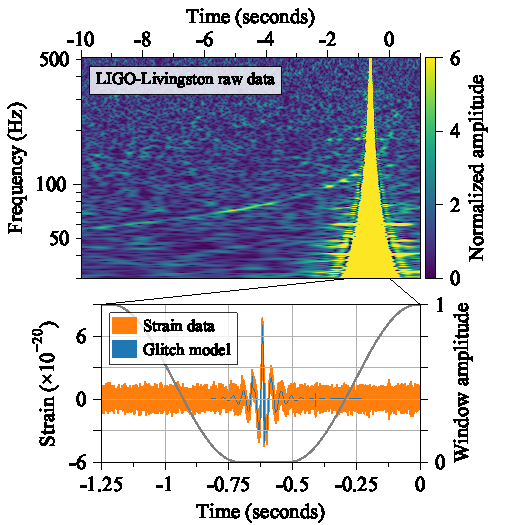
\includegraphics[width=1.0\linewidth]{images/6_earlywarning/gw170817/GW170817_glitch_subtraction.pdf}
    \caption{The Q-scan of the LIGO-Livingston data containing GW170817, with a very loud wide bandwidth glitch present (top). The glitch was initially subtracted from the data using a windowing function to reduce the amplitude of the glitch to $0$, this windowing function can be seen as a grey line in the bottom figure. The glitch was also modelled using Bayeswave~\cite{BayesWave:2015} and subtracted from the data to preserve the gravitational wave signal power found beneath the glitch, this glitch model (blue line) can be seen overlapping the strain data (orange line) in the bottom figure. This figure has been taken from~\cite{GW170817:2017}.}
    \label{6:fig:gw170817_glitch}
\end{figure}
%

We now have more robust and well tested search pipelines which are capable of finding gravitational wave events with a maximum latency of $20$ seconds post-merger~\cite{PyCBC_Live:2018}, with the ability to rapidly make sky maps using BAYESTAR~\cite{BAYESTAR:2016} and have the ability to auto-gate any loud glitches in the data. Assuming the BAYESTAR sky map is good enough and there are enough detectors to effectively cover the whole sky map (we have instruments such as GOTO which are used specifically for gravitational wave event followup~\cite{GOTO:2020}), gamma-ray bursts can arrive less than two seconds after the gravitational wave merger. This is not nearly enough time to produce a sky map or relocate a telescope. As an example, the PyCBC Live full-bandwidth gravitational wave search has a maximum latency between detection and upload to GraceDB of $20$ seconds, as shown by figure~\ref{6:fig:latency_plot}.
%
\begin{figure}
    \centering
    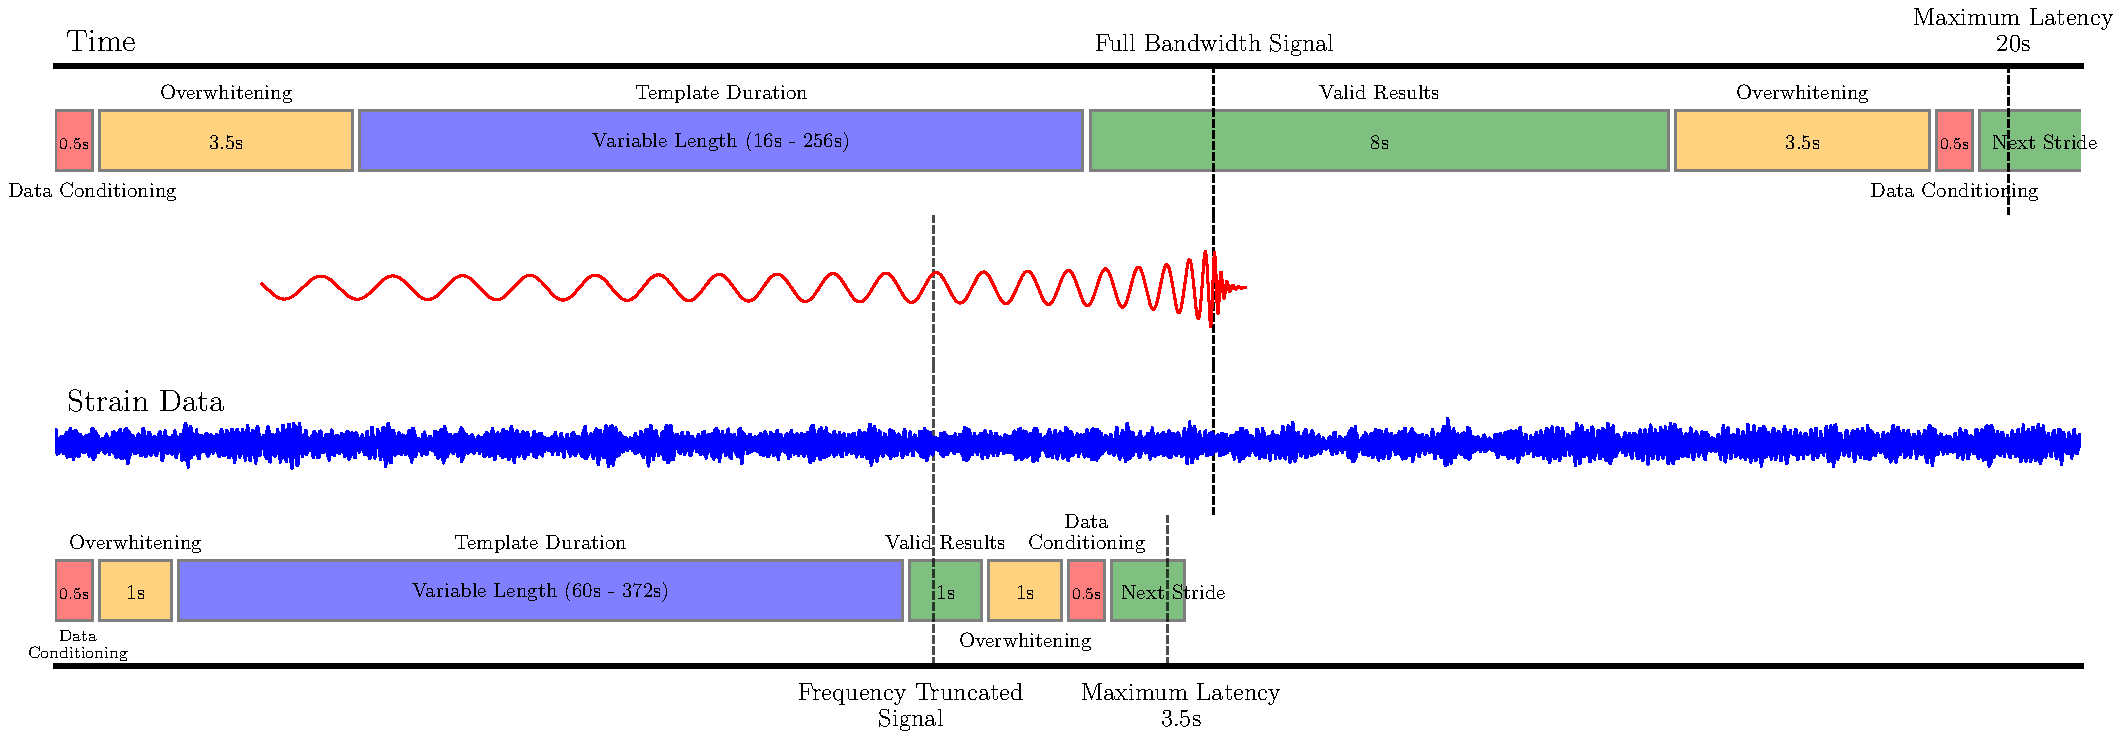
\includegraphics[width=\textwidth]{images/6_earlywarning/gw170817/latency_plot.pdf}
    \caption{}
    \label{6:fig:latency_plot}
\end{figure}
%
An early warning search will search for pre-merger gravitational wave signals. When one has been found it can estimate the time of coalescence, produce a sky map, and send out an alert to the international astronomy community to be prepared for an incoming gravitational wave merger. The details of the PyCBC Live early warning search will be covered in this chapter.

We can demonstrate the early warning search's efficacy on GW170817. Table~\ref{6:tab:gw170817_early_warning} displays a selection of frequencies alongside the network SNR of the early warning search in both the original data and a representation of the current detector data, also shown is the time pre-merger (latency) at which GW170817 will reach the specified frequency. It can be clearly seen that the SNR of the early warning search hovers around the network SNR threshold of $6$ until the $56$Hz frequency is reach, it is at this point that we can more confidently say that GW170817 would've been seen in early warning, $12$ seconds prior to the merger. When we inject a GW170817-like signal into O4 data we can see very large SNRs in all of the frequencies and the earliest we could observe an early warning signal from GW170817 would be $67$ second prior to the merger.
%
\begin{table}[ht]
    \centering
    \setlength{\tabcolsep}{4pt}
    \rowcolors{4}{white}{lightgray}
    \begin{tabular}{cccc}
        \toprule
        & \multicolumn{2}{c}{\textbf{Network SNR}} & \\
        \cmidrule(lr){1-4}
        \textbf{Final Frequency [Hz]} & \textbf{Original Data} & \textbf{O4 Injection} & \textbf{Time Pre-Merger [s]} \\
        \midrule
        29 & 6.19 & 13.26 & 67 \\
        32 & 5.76 & 18.58 & 52 \\
        38 & 6.11 & 21.96 & 33 \\
        44 & 6.25 & 25.87 & 22 \\
        49 & 6.19 & 24.42 & 17 \\
        56 & 7.04 & 35.24 & 12 \\
        \bottomrule
    \end{tabular}
    \caption{Caption text goes here}
    \label{6:tab:gw170817_early_warning}
\end{table}
%
By implementing an early warning search in PyCBC Live we are capable of identifying gravitational signals before merger. This will aid in localising potentially electromagnetically bright gravitational wave signals and inform telescopes of all frequency ranges around the globe and in space to capture as much of the electromagnetic counterpart as possible, enabling greater quality multi-messenger astronomy.

\section{Early Warning Search}

PyCBC Live has two currently active configurations running on real gravitational wave data in real time: the full-bandwidth search aims to identify all gravitational wave signals in the data in low-latency; the early warning search aims to identify potentially electromagnetically bright signals prior to their merger.

The PyCBC Live full bandwidth and early warning searches use the same infrastructure and code. The full bandwidth search uses a data stride of eight seconds, meaning new data is loaded every eight seconds, while the early warning search has a data stride of one second. As shown in on the top of figure~\ref{6:fig:latency_plot} the full bandwidth search has a minimum and maximum latency of 12 and 20 seconds respectively between gravitational wave merger and PyCBC Live detection, the corresponding figure for the early warning search is shown on the bottom of figure~\ref{6:fig:latency_plot}, where we can see that we have a minimum latency between initial gravitational wave detection of 2.5 seconds and a maximum latency of 3.5 seconds but between initial detection of the lowest frequency being searched for.

The clear difference between the two searches is the ability for the early warning search to detect gravitational wave signals prior to merger using templates which have been truncated a specific frequencies. When a significant amount of SNR has been accumulated in the inspiral region we can detect the signal and predict the time of merger, and with multiple templates for the same signal at different final frequencies we can build up a signal and report multiple events for the same gravitational wave signal. We are even able to make preliminary sky maps from these frequency truncated events, with the sky map becoming more and more accurate as more SNR is accumulated in higher final frequency events.

\section{Template Bank}

The PyCBC Live early warning search uses a frequency truncated template bank to search for gravitational wave signals prior to merger. The full bandwidth gravitational wave templates are generated with the \verb|TaylorF2| waveform model which models the inspiral region of the signals and is unable to accurately model the merger phase, this is acceptable because these low mass signals merge above the upper frequency band of detector sensitivity. The frequency evolution of the inspiral region of \verb|TaylorF2| waveforms is monotonic in time, meaning a specific time before merger corresponds directly to a particular frequency to truncate to. Therefore to observe a template $30$ seconds pre-merger, we can map that directly to a frequency and trunacate the template at that frequency. This is even easier when we consider that \verb|TaylorF2| waveforms are frequency domain so no conversion between time and frequency is required.

The current bank we use has truncated frequencies of \verb|29, 32, 38, 44, 49, 56| which match the grid of frequencies used by the other early warning searches of the pipelines: GstLAL~\cite{GstLAL:2020}, MBTA~\cite{MBTA:2021} and SPIIR~\cite{SPIIR:2020}. These templates correspond to roughly \verb|60, 46, 29, 20, 15, 10| seconds before merger for a $1.4M_\odot$-$1.4M_\odot$ BNS signal. The bank is constructed by generating a template bank using the standard geometric placement algorithm~\cite{Brown:2012} and a minimal match of $0.97$ for each frequency cutoff and then combining the six template banks into one.

The template parameters themselves are chosen to represent potentially electromagnetically bright, low mass BNS or NSBH systems. This means that a single full bandwidth signal isn't simply generated and split into six frequency truncated templates and in fact a full bandwidth template might not have six frequency truncated templates that exactly match but they are covered by a nearby template with a minimum match of $0.97$. The masses of the two systems are limited between $1-3 M_\odot$, with no spins. The PSD used to generate the template bank is \verb|aLIGO140MpcT1800044| which is a representative PSD of the Advanced LIGO design curve that includes estimates for the main fundamental noises of the interferometer, in particular: seismic noise, thermal noise and quantum noise~\cite{aLIGO_design_curve:2018}. Using this PSD as our noise model will mean the data contains no non-Gaussian noise artefacts.

The complete early warning template bank is $9180$ templates, making for a very light weight search computationally when compared to the ~$700,000$ templates being used in the full bandwidth PyCBC Live search. Not only are there a smaller number of templates in the template bank, the templates themselves are shorter in duration when compared to their full bandwidth counterparts in the full bandwidth template bank.
%
\begin{figure}
    \centering
    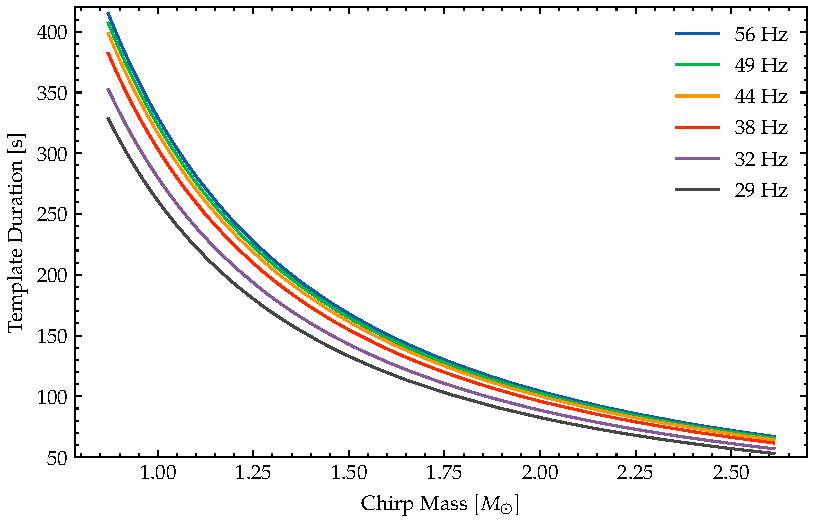
\includegraphics[width=\textwidth]{images/6_earlywarning/search/template_bank_duration_mchirp.pdf}
    \caption{Template duration versus Chirp mass, $\mathcal{M}$, for different final frequency cuts in the early warning template bank. Each curve corresponding to a different final frequency, $f_{final}$, (ranging from 29 Hz to 56 Hz). The chirp mass is calculated from the component masses of the binary system, and the template duration is from $17$ Hz to $f_{final}$ Hz).}
    \label{6:fig:tb_duration_mchirp}
\end{figure}
%
The duration of templates at each final frequency cutoff can be seen in figure~\ref{6:fig:tb_duration_mchirp} as a function of the chirp mass, $\mathcal{M}$, of the template. It can be seen that higher $\mathcal{M}$ templates have shorter durations and templates with lower final frequency cutoffs also have lower durations when compared to templates with the same $\mathcal{M}$ but a higher final frequency.

\section{Event Localisation}

% (BRILLIANT PAGE FOR THIS https://emfollow.docs.ligo.org/userguide/early\_warning.html)

We have previously mentioned the ability for the early warning search to provide a preliminary sky map of an event to aid in localisation pre-merger when passing information to the wider scientific community for followup in the multi-messenger regime. To demonstrate the sky map localisation as the signal progresses through our template bank we can perform a test using a representative $1.4M_\odot$-$1.4M_\odot$ BNS signal at a random point on the sky, and a few different distances, and evaluate the sky maps produced by BAYESTAR.


%%%% REWRITE ALL OF THIS
We produce the $1.4M_\odot$-$1.4M_\odot$ BNS signal and scale the distance so that it will be seen with a full-bandwidth SNRs of: $10$, $20$, $30$. Then we search for these signals with the early warning search and for each candidate produced by the search we look at the sky map and the number of \verb|degrees|$^2$ in the 50\% credible area to see how the signal becomes more localised as more of the signal is being seen. We plot injection as a star on the sky maps and the $50\%$ confidence interval contours are plotted for each final frequency event belonging to the same injection on the same sky map, these can be seen in figure~\ref{fig:ew_10SNR_multiple} for the 10 SNR injection, figure~\ref{fig:ew_20SNR_multiple} for the 20 SNR injection and, figure~\ref{fig:ew_30SNR_multiple} for the 30 SNR injection. A table has also been produced containing the sky localisation area for each final frequency event for each of the injections, table~\ref{tab:ew_inj_skymaps}.
% Keep only the example sky map for 30 SNR but keep the others in the table
%
% \begin{figure}
%     \centering
%     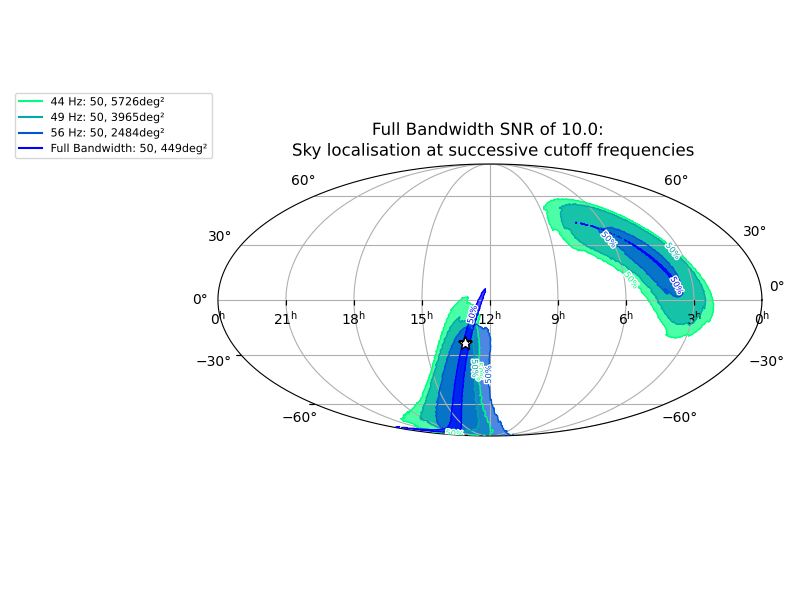
\includegraphics[width=\textwidth]{images/6_earlywarning/localisation/10SNR_multiple.png}
%     \caption{}
%     \label{fig:ew_10SNR_multiple}
% \end{figure}
%
% \begin{figure}
%     \centering
%     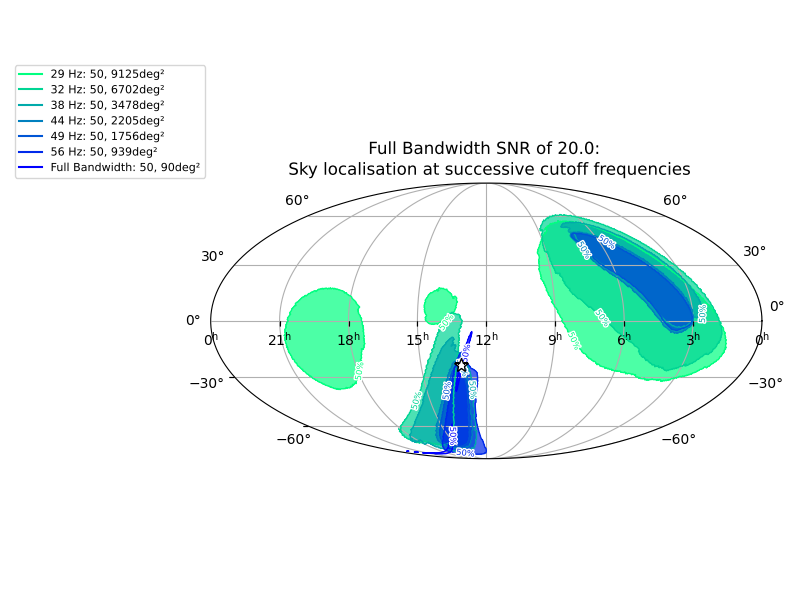
\includegraphics[width=\textwidth]{images/6_earlywarning/localisation/20SNR_multiple.png}
%     \caption{}
%     \label{fig:ew_20SNR_multiple}
% \end{figure}
%
\begin{figure}
    \centering
    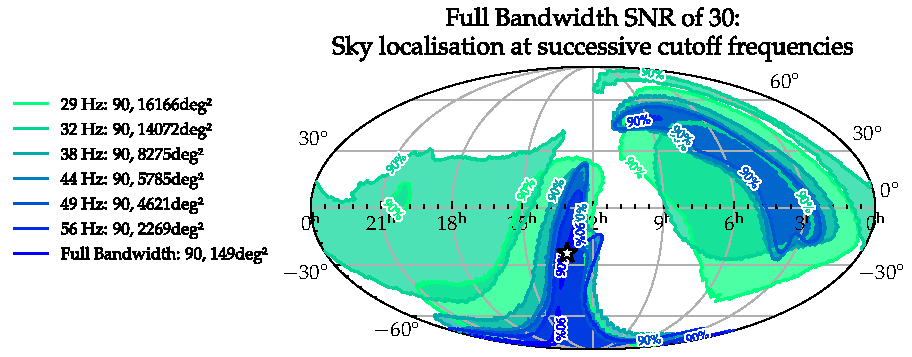
\includegraphics[width=\textwidth]{images/6_earlywarning/localisation/30SNR_multiple.pdf}
    \caption{The gravitational wave sky localisation probability map (sky map) corresponding to a $1.4$M$_{\odot}$-$1.4$M$_{\odot}$ binary neutron star signal with a full-bandwidth (upper frequency cutoff $= 1024$Hz) signal-to-noise ratio of $30$. The successive $90\%$ confidence interval sky map contours for final frequency cutoffs from $29-56$Hz are shown where it can be seen that a higher final frequency cutoff leads to a more constrained sky map.}
    \label{6:fig:ew_30SNR_multiple}
\end{figure}
%
\begin{table}[ht]
    \centering
    \setlength{\tabcolsep}{4pt}
    \rowcolors{4}{white}{lightgray}
    \begin{tabular}{cccc}
        \toprule
        \textbf{Final SNR} & \textbf{10} & \textbf{20} & \textbf{30 (Fig.~\ref{6:fig:ew_30SNR_multiple})} \\
        \midrule
        \textbf{Frequency [Hz]} & \multicolumn{3}{c}{\textbf{Localization accuracy [deg$^{2}$] (90\% credible area) }} \\
        \cmidrule(lr){2-4}
        29 & Not Found & 26,583 & 16,166 \\
        32 & Not Found & 22,464 & 14,072 \\
        38 & Not Found & 12,303 & 8,275 \\
        44 & 18,584 & 8,408 & 5,785 \\
        49 & 14,068 & 6,758 & 4,621 \\
        56 & 9,636 & 4,679 & 2,269 \\
        1024 & 1,908 & 300 & 149 \\
        \bottomrule
    \end{tabular}
    \caption{Caption text goes here}
    \label{6:tab:gw170817_early_warning}
\end{table}
%
It is the case, especially for the low SNR signal, that the injection at every final frequency cutoff. Figure~\ref{fig:ew_10SNR_multiple} is missing the \verb|29, 32| and \verb|38| Hz events. It is very clear to see in table~\ref{tab:ew_inj_skymaps} that a higher SNR directly translates to a better sky localisation. The 30 SNR injection has been constrained sky maps at all frequencies.

DESCRIBE THE SKY MAPS AND THE CONTOUR INTERVALS. 50\% REFERS TO THE SMALLEST AREA ON THE SKY, MINIMIZED. FIND OUT HOW THIS IS DONE. 

\section{Injection Runs in Offline}

To investigate the efficacy of the early warning search I performed an injection campaign very similar to the injection campaigns done in the previous chapters~\ref{chapter:4-archenemy} and~\ref{chapter:5-pycbc-live}. To test the early warning search the injection set was custom generated to include exclusively signals that should be seen by the early warning search, instead of the injection sets used in the third observing run~\cite{gwtc3:2023}.

\subsection{Injection Set \& Data}

The injection set contains 32,604 unique injections placed every $\sim100$ seconds, encompassing 3,456,000 seconds or exactly 40 days worth of data. The parameters which vary by injection and the ranges in which they vary can be seen in table~\ref{6:tab:ew_inj_params}.
%
\begin{table}[ht]
    \centering
    % \small
    \setlength{\tabcolsep}{4pt}
    \rowcolors{2}{white}{lightgray}
    \begin{tabular}{ccc}
        \toprule
        \multicolumn{3}{c}{\textbf{Variable Parameters}} \\
        \cmidrule(lr){1-3}
        \textbf{Parameter} & \textbf{Value Range} & \textbf{Prior Distribution} \\
        \midrule
        Primary Mass, $m_1$ & 1.0 - 3.0 [$M_{\odot}$] & uniform \\
        Secondary Mass, $m_2$ & 1.0 - 3.0 [$M_{\odot}$] & uniform \\
        Primary Spin z-component, $spin1z$ & -0.05 - 0.05 & uniform \\
        Secondary Spin z-component, $spin2z$ & -0.05 - 0.05 & uniform \\
        Distance, $r$ & 10 - 1000 [$Mpc$] & uniform radius \\
        Phase, $\phi_{c}$ & - & uniform angle \\
        Inclination, $\iota$ & - & sin angle \\
        Polarization, $\psi$ & - & uniform angle \\
        Right Ascension, $\alpha$ & - & uniform sky \\
        Declination, $\delta$ & - & uniform sky \\
        \bottomrule
        \multicolumn{3}{c}{\textbf{Static Parameters}} \\
        \cmidrule(lr){1-3}
        \textbf{Parameter} & \textbf{Value} & \textbf{} \\
        \midrule
        Waveform Approximant & IMRPhenomXAS & \\
        Lower Frequency, $f_{lower}$ & 17 [$Hz$] & \\
        Reference Frequency, $f_{ref}$ & 17 [$Hz$] & \\
        \bottomrule
    \end{tabular}
    \caption{Caption text goes here}
    \label{6:tab:ew_inj_params}
\end{table}
%
These injections are made into simulated noise with no non-Gaussian artefacts or non-stationarity and a constant PSD. The distances generated for each injection are re-scaled after the initial injection set has been created to ensure a uniform SNR distribution of the signals between $12$ and $60$. Therefore the distances might not be exactly uniform in radius and the injection set should be thought to be distributed uniformly in SNR instead.

\subsection{Results}

% TO ADD:
% - Basic stats about results
% - Number of injections
% - Number of candidates found
% - Histogram/Table of candidates per injection
% - SNR distributions for candidates for frequencies
% - 

Each injection has the potential to be seen by six different templates and therefore we might expect to see exactly six times the number of injections in the data. However, for the very low final frequency templates in the bank (29Hz) these would require at least 4 (DOUBLE CHECK) SNR (the SNR threshold for detection) to be accumulated in a very small frequency window, which is very unlikely for the 12 SNR injections but possible for our 60 SNR injections. (CHECK THIS TO SEE WHAT THEY ACTUALLY FOLLOW, MINIMUM SNR FOR 29Hz DETECTION)

Another reduction in the number of candidates found will be caused by a very short time gap between final frequencies 49Hz and 56Hz. The evolution of the gravitational wave signals inspiral increases over time and therefore these two frequencies might be found within a stride and therefore one will be skipped. These two effects will cause a reduction in the total number of candidates seen by this injection test.

The total number of candidates found for all injections is (NUMBER). 

PyCBC Live outputs the candidates found during the search and outputs the time of coalescence of the non-truncated template. Therefore, even if a 29Hz template finishes many seconds before time of coalescence of the gravitational wave signal, we can collect all of the candidates associated with an injection by comparing injection time and time of coalescence of candidates. We look for candidates with a time of coalescence within +-0.5 seconds of the injection time, this ensures that we are looking for candidates which have all been predicted to end in the same search stride.

Figure~(REF) shows a histogram of the number of candidates found per injection. (INSERT THE FIGURE)

\section{\label{6:sec:identified-problems}False alarms, missed injections and other problems}

Previous injection tests in this thesis were performed to measure sensitivity increases from significant changes to the gravitational wave search pipelines. The injection test performed on the PyCBC Live Early Warning search was not intended to measure sensitivity increase but to identify problems that might occur with the search that can only be seen by a large number of injections in testing. Performing this injection test will help us identify, investigate and solve problems to the Early Warning search prior to them occurring during the live operation of the Early Warning search where we might miss a real event.

In this section we will identify problems discovered during the Early Warning injection test. These problems are their impact on the search results will be described and the source of the problem (where identified) will be detailed. Where possible the solution to these problems will also be discussed.

\subsection{\label{6:sec:false-alarms}False-alarm events}

False-alarms are events for which the coincident triggers have originated from non-astrophysical sources to form a candidate found above our statistic threshold. It is easier to identify false-alarm early warning events because those that appear at a lower frequency will not have the corresponding candidates from the next frequencies in the template bank. This is not something the early warning search can take into account in low-latency but it is something that can definitely be used post-detection to confirm the legitimacy of an event.

We can identify false-alarm events in our results by locating candidates which appear with a time of coalescence outside of a short window surrounding any injections times in our injection set.

\subsubsection{\label{6:sec:low-significance-cands}Low significance individual candidates}
%
\begin{figure}
       \centering
    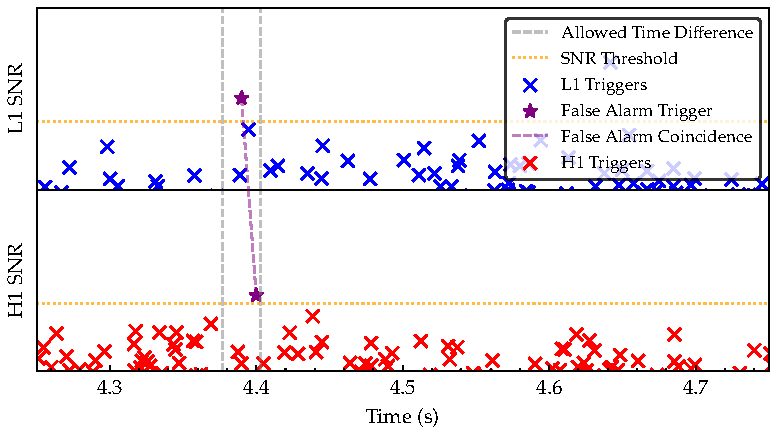
\includegraphics[width=\textwidth]{images/6_earlywarning/identified-problems/low_sig_cands.pdf}
    \caption{}
    \label{6:fig:low_significance_candidates}
\end{figure}
%
The injection set used in this search was made using a PSD representative of the advanced LIGO noise curve~\cite{aLIGO_design_curve:2018} and therefore is coloured Gaussian noise, not containing any non-Gaussian noise transients. This means that when we identify a false-alarm candidate it has been caused by Gaussian noise triggers aligning in between the two detectors and finding a coincidence, a demonstration of this can be seen in figure~\ref{6:fig:low_significance_candidates}.

In the early warning search we have a lower SNR threshold on single detector triggers of $4.5$.

We allow a false-alarm rate of X for the early warning search, therefore, for $40$ days of data we might expect to see Y number of false-alarms.

Here is the maths for calculating the actual likelihood for a false-alarm when dealing with a simple statistic of noise rate only, with quadsum.
% - Example
% - How often it happened
% - Impact





\subsection{\label{6:sec:duplicate-frequency-cands}Duplicate final frequency candidates found for one injection}

% Lay out the problem
%  Injections seen with more than 6 events
%  Injections can only be seen with $6$ max
%  What is happening?
%  Some frequencies are seen twice
%  What?? How can that happen if the search picks the best coincidence in the second that corresponds to the final frequency truncation?

The template bank used by the early warning search is a composite of six template banks. Each template bank contains templates which all end at the same final frequency cutoff and is different for each template bank. Therefore, the full template bank contains templates for six different final frequency cutoffs.

The time before merger corresponding to each frequency cutoff is then injection specific and you would expect that when the early warning search reaches that time, it would record an event found by a template with the correct final frequency cutoff. This then places a maximum number of events found for each injection using the template bank at six events.

We have however, observed injections that have been seen with more than six candidate events. These candidates must have final frequency cutoffs equal to one of the six found in our template bank and therefore some frequency cutoffs have been found multiple times for an injection. This should not be possible as the time before merger for the frequency cutoff would correspond to a stride in the early warning search and only the best coincident event can be chosen by the early warning search as a candidate.

\subsubsection{\label{6:sec:cands-across-bounds}Candidates straddling search boundaries}
%  Well, some truncations are close to the boundary
%  Others are across the boundary
%  There is enough lee-way to pick two in two separate seconds
%
\begin{figure}
       \centering
    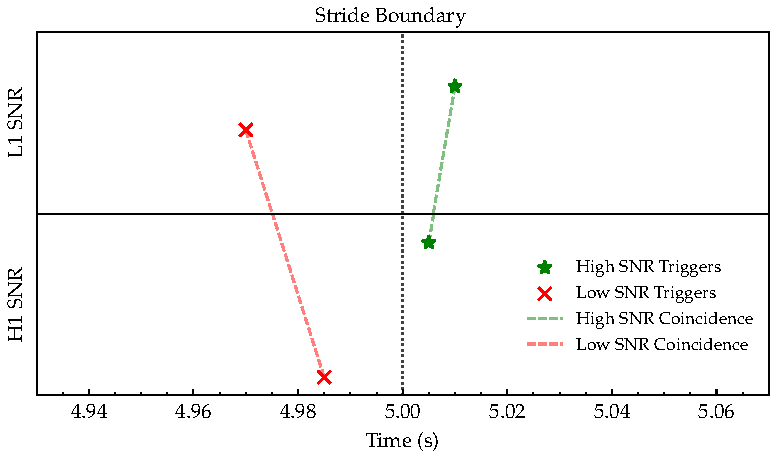
\includegraphics[width=\textwidth]{images/6_earlywarning/identified-problems/cands_across_bounds.pdf}
    \caption{}
    \label{6:fig:candidates_across_boundaries}
\end{figure}
%

The early warning search operates on a single second stride, meaning every single second the template bank is matched filtered with the data to discover any gravitational wave events. It is possible that the pre-merger time corresponding to a final frequency cutoff will lie very near to the boundary between search strides. In this case the search will record an event found in the first stride and will then again record another event in the second stride with the same final frequency cutoff.

Figure~\ref{6:fig:candidates_across_boundaries} is a demonstration of this possibility. Either event can have a higher SNR when compared to the other but the two scenarios can be treated differently to prevent some duplicate events being uploaded in the future. If the event found in the first stride has a higher SNR than the second stride we can prevent an upload of the second event (provided the template final frequencies are the same)---this is already done by the PyCBC Live Single Detector search~\cite{PyCBC_singles:2022}---but if the event found in the second stride has a higher SNR than the first then we will have to upload two events. We cannot delay uploading the first event.

% Maybe an example of this happening with a zoom in on the two duplicate frequencies in the track and trigger times, stride boundary time, event time, things like that
% - Example
% - How often it happened
% - Impact



\subsubsection{\label{6:sec:trigs-across-bounds}Triggers across search boundaries}
%  The search forces a coincidence in the first seocnd and then finds the actual one in the second second
%
\begin{figure}
       \centering
    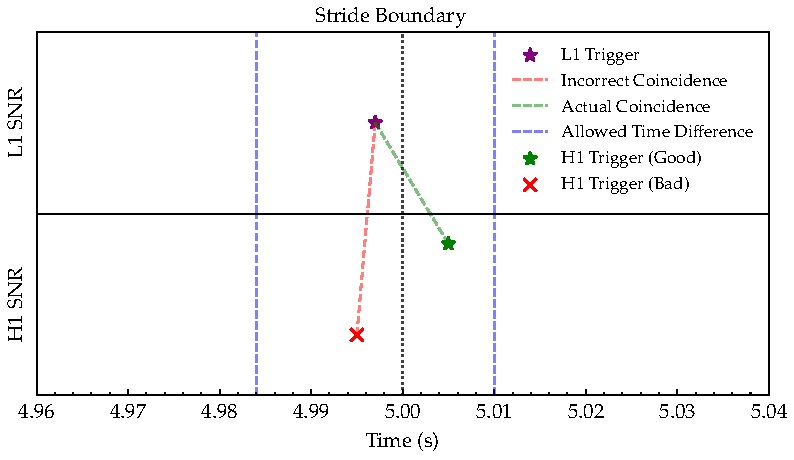
\includegraphics[width=\textwidth]{images/6_earlywarning/identified-problems/trigs_across_bounds.pdf}
    \caption{}
    \label{6:fig:triggers_across_boundaries}
\end{figure}
%
The stride boundary can have another effect which causes duplicate frequency events to be uploaded. Coincident triggers between detector 1 and detector 2 have an allowed time difference in each detector to account for the physical light-travel time of the gravitational wave and a smaller amount of computational timing errors. It is possible for the two single detector triggers to appear across a stride boundary.

The trigger will first be seen in detector 1, which will be seen as a highly significant single detector trigger by the early warning search, where it will attempt to match with a coincident trigger in the other detector. As previously mentioned, this could be Gaussian noise which happens to match well enough for a low-significance coincidence to be made. When detector 2 records the trigger in the next stride the early warning search will create the actual significant coincident event using the same detector 1 trigger twice. Therefore, we will get two candidate events at the same final frequency cutoff with one being less significant than the other. A demonstration of this case is seen in figure~\ref{6:fig:triggers_across_boundaries}. This is unavoidable, we need the light travel time in the ranking statistic and this can straddle two strides.

% Example once again of the same trigger being used for both events? H1 SNR the same, L1 snr different (much lower and much higher)
% - Example
% - How often it happened
% - Impact




\subsection{\label{6:sec:outside-coinc-window}Coincident triggers outside the light-travel time}
%
\begin{figure}
    \centering
    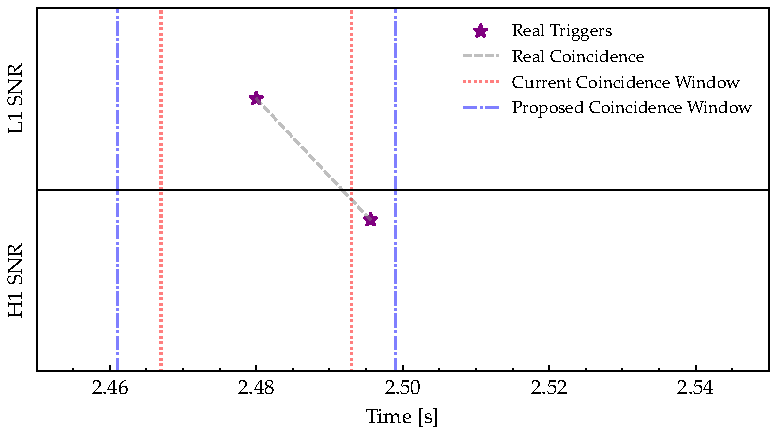
\includegraphics[width=\textwidth]{images/6_earlywarning/identified-problems/outside_coinc_window.pdf}
    \caption{Caption}
    \label{6:fig:outside_coinc_window}
\end{figure}
%
% What is the broad problem?    
% What are some ways it manifests
% How can we solve this problem
%  Coinc Window - Fairhurst
%  PhaseTD tuning for statistic
%  Sample rate issue

A problem that we have identified in the analysis of the results is valid candidates events being missed due to the coincident triggers falling outside of the allowed coincidence time window. The coincidence time window is a sum of the light-travel time and a computational timing error allowance. The two LIGO detectors are separated by a straight line through the Earth $3002$ kilometers long. Given the speed of light, c $= 300,000$ km/s, there is a $0.01$ window and the current addition for errors is $0.003$ seconds, giving a total allowed coincidence timing window of $0.013$ seconds. How then, is it possible for our completely valid coincident triggers to lie outside of this window?

\subsubsection{\label{}Timing accuracy error}

Firstly, as described in~\cite{Fairhurst:2010}, the accuracy of the candidate time in a detector can be determine by,
%
\begin{equation}
    \sigma_{t} = \frac{1}{2\pi\rho\sigma_{f}}
    \label{6:eqn:timing_acurracy}
\end{equation}
%
where the timing accuracy, $\sigma_{t}$, is inversely propertional to the SNR, $\rho$, and the effective bandwidth of the source, $\sigma_{f}$ which is defined as
%
\begin{equation}
    \sigma_{f}^2 = \left(\frac{4}{\rho^{2}} \int^{\infty}_{0} df \frac{f^{2}|h(f)|^{2}}{S(f)}\right) - \left(\frac{4}{\rho^{2}} \int^{\infty}_{0} df \frac{f|h(f)|^{2}}{S(f)}\right)^{2} .
    \label{6:eqn:eff_bandiwdth}
\end{equation}
%
As shown in Table 1. of~\cite{Fairhurst:2010}, the timing error for a binary neutron star system in an advanced LIGO configuration with a BNS range of $160$ Mpc is $0.46$ms. Negligible when compared to our light-travel time of $10$ms. We can perform an approximately calculate the timing accuracy of the early warning templates using equations~\ref{6:sec:duplicate-frequency-cands} \&~\ref{6:eqn:timing_acurracy}, where the gravitational wave strain term, $|h(f)|$, is assumed to be equal to the inspiral frequency evolution of a binary neutron star signal, $f^{-\frac{7}{6}}$. The estimated effective bandwidths and timing accuracy errors can be seen in table~\ref{6:tab:timing_errors}.
%
\begin{table}[ht]
    \centering
    \setlength{\tabcolsep}{4pt}
    \rowcolors{3}{white}{lightgray}
    \begin{tabular}{ccc}
        \toprule
        \textbf{Frequency [Hz]} & $\sigma_{f}$ [Hz] & $\sigma_{t}$ [ms] \\
        \midrule
        29 & 0.51 & 6.80 \\
        32 & 0.57 & 6.49 \\
        38 & 0.66 & 6.00 \\
        44 & 0.74 & 5.61 \\
        49 & 0.79 & 5.35 \\
        56 & 0.86 & 5.05 \\
        1024 & 2.98 & 1.66 \\
        \bottomrule
    \end{tabular}
    \caption{Caption text goes here}
    \label{6:tab:timing_errors}
\end{table}
%
Using an SNR of $8$ (and a lower frequency of $17$ Hz) yields timing errors from $6.80$ to $5.05$ milliseconds for the early warning final frequency cutoffs, where higher frequencies have a smaller timing error. These values are the same order of magnitude as the light-travel time ($10$ms) and therefore need to be considered in the early warning search to ensure we are identifying coincidences.

\subsubsection{\label{}Sampling accuracy}
% PyCBC Live Full Bandwidth Sample Rate
%  Why does it need a high sample rate
% PyCBC Live Early Warning Sample Rate
%  Why is it lower
%   To capture the f_final in the nyquist
%  Why isn't it even lower?
%   You lose out on time and phase resolution
%  How is this affecting our search
%   Triggers in between two samples can be found outside the coincident time window

The PyCBC Live Full Bandwidth uses a sample rate of $2048$Hz to capture binary neutron star signals which can merge even above the $1024$Hz Nyquist frequency with the greatest accumulated SNR. The PyCBC Live Early Warning search uses a sample rate of $256$Hz, giving a Nyquist frequency of $128$Hz. The highest final frequency cutoff templates are at $56$Hz so these can all be fully captured with a sample rate of $128$Hz. The sample rate is increased to $256$Hz to ensure we have a greater time resolution and phase accuracy, a sample rate of $128$Hz has a time between samples of $7.8$ms which is close to our allowed light-travel time.

We have seen that the $256$Hz sample rate might still provide an issue with timing accuracy and the current allowed coincidence time window. With a time between samples of $3.9$ms a trigger in another detector $3$ samples later will be within the allowed window of $13$ms but $4$ samples which equal a time difference of $15.6$ms, outside the window. We have seen examples whereby increasing the sample rate of the early warning search will locate a coincidence within the time window where previously it was seen outside. Increasing the sample rate however, does increase the computational cost of the search with no increase in event SNR or new events provided.

\subsubsection{\label{}Early warning tuned PhaseTD histogram}
% Great, we've made the window bigger
% What? It still won't work? Why not?
% PhaseTD File
%  What is it?
%  How is it made?
%  How is it tuned?
%  Does it take into account time windows outside the 13ms? (no)

By increasing the allowed coincidence time window we will allow the early warning search to make those initial coincident triggers which share the same template parameters and are physically possible (when accounting for timing accuracy error). However, we will face another problem where the coincident ranking statistic used by the early warning search will not consider these event to have a very low signal rate. The coincident ranking statistic used by the early warning search is \verb|phasetd| (phase-time delay) and is used to assess the coincidence likelihood between two triggers from different detectors.

For a two detector coincidence the likelihood value is found by sampling from a pre-created \verb|phasetd| 3-dimensional histogram in amplitude, time and phase space. This file is created using by simulating gravitational wave signals from an isotropic distribution of sources. Each signal is assigned a random sky location (right ascension, declination and inclination) and polarization, then the response in each detector is calculated to determine the sensitivity to the signal in both detectors. From this response we can get the signal amplitudes, time delays and phases shifts for each detector. For the pair of detectors the time delay, phase differences and relative signal amplitudes are then binned into discrete bins which represent different combinations of amplitude, time and phase difference.

The size of the bins is determined by the allowed uncertainties in timing, phase and SNR. Additionally there is a restriction in the allowed range of SNR ratios to avoid storing bins for extreme values. After this, smoothing is performed between nearby bins and the final histogram is produced. Within the search, time difference, phase difference and amplitude ratios are then used to sample from this histogram to calculate the likelihood of the three parameter combination.

Currently the allowed time window uncertainty is $1$ms which determines the bin size and while the time difference between two triggers is allowed to include these early warning trigger coincidences in our monte carlo simulation of of the astrophysical distribution of these time differences the early warning time difference bins will not be occupied due to these lying outside of the light-travel time. The uncertainty will need to be taken account explicitly in the time difference on both trigger times.

Another improvement that can be made in the generation of the \verb|phasetd| statistic files is including the sample rate of the search as a parameter. For a monte carlo simulation our sample rate is as accurate as a \verb|float64| parameter can be. Whereas the timing difference between triggers in the PyCBC Live search will only take discrete values of the time difference dependent on the sample rate, for example, the early warning search has a sample rate of $256$Hz and therefore the time difference between samples is $0.00390625$ seconds or approximately $3.9$ milliseconds. Therefore our \verb|phasetd| file will only ever been sampled from using time difference that are n-multiples of this time between samples. We can create \verb|phasetd| files with bins in the time difference parameter space which represented the sample rate of the search and therefore can be sampled more accurately.

\subsubsection{\label{6:sec:missing-cands}Missing candidates}
%
\begin{figure}
       \centering
    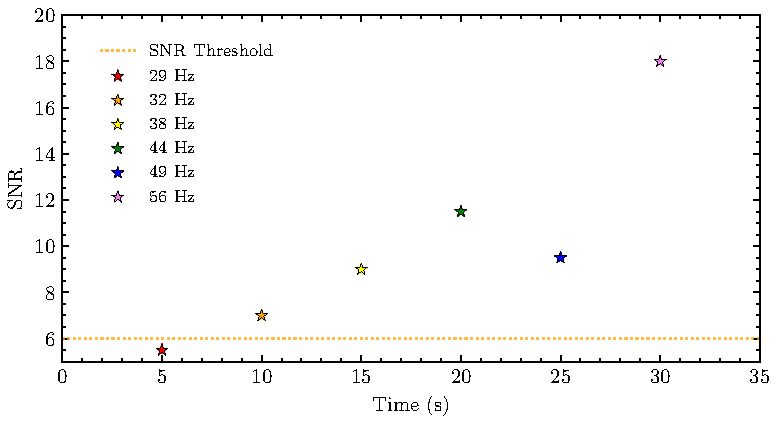
\includegraphics[width=\textwidth]{images/6_earlywarning/identified-problems/non_mono_snr.pdf}
    \caption{}
    \label{6:fig:non-monotonic-snr}
\end{figure}
%
% - Example
% - How often it happened
% - Impact

The most obvious indicator that the search has failed to find a coincidence due to the coincident trigger time difference falling outside the coincidence allowed timing window is that injections have `missing' events in the frequency evolution. We would expect to see a sequence of events for each injection when the starting frequency is not the greatest frequency truncation in the bank. For example, if we saw a real candidate event with a final frequency cutoff of $29$Hz then we would expect to find the $32$, $38$, $44$, $49$ and $56$Hz candidate events shortly following. If we fail to see the $32$Hz event but we still see the following events then we know that something has broken in the early warning search.

We know that the $32$Hz triggers exist but they fall outside the allowed coincidence timing window and therefore a coincident event was never formed. The early warning search will output files containing all the single detector triggers found which we can use to identify the missing coincidence. Figure~\ref{6:fig:missing-freq-eg} shows an example of an injection which has been found with all but $1$ final frequency cutoff template. 
%
\begin{figure}
    \centering
    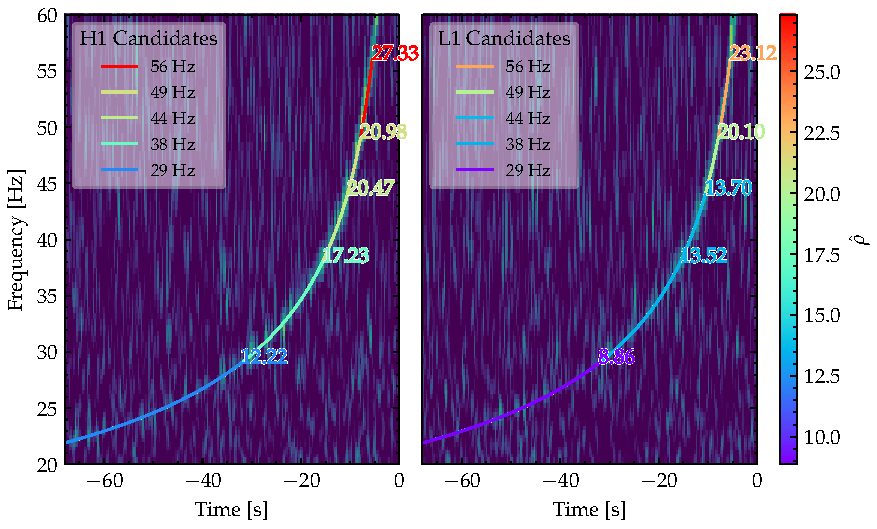
\includegraphics[width=1.0\linewidth]{images/6_earlywarning/stories/missing_freqs_example.pdf}
    \caption{Caption}
    \label{6:fig:missing-freq-eg}
\end{figure}
%
To verify the time difference problem we investigated the expected network SNRs for this injection at each final frequency cutoff in both a noiseless and expected noise regime (not performed using the PyCBC Live search). The values for these can be seen in table~\ref{6:tab:noise_snrs}.
%
\begin{table}[ht]
    \centering
    \setlength{\tabcolsep}{4pt}
    \rowcolors{2}{white}{lightgray}
    \begin{tabular}{ccc}
        \toprule
        \textbf{Final Frequency [Hz]} & \textbf{Noiseless SNR} & \textbf{Noisy SNR} \\
        \midrule
        29 & 16.43 & 15.38 \\
        32 & 19.16 & 17.95 \\
        38 & 24.00 & 21.50 \\
        44 & 28.11 & 25.26 \\
        49 & 31.04 & 27.94 \\
        56 & 34.48 & 29.02 \\
        \bottomrule
    \end{tabular}
    \caption{Caption text goes here}
    \label{6:tab:noise_snrs}
\end{table}
%
We can clearly see that we are expecting to see a large network SNR for the $32$Hz case which isn't recovered by the PyCBC Live Early Warning search. Next we are able to re-run the early warning search using a template which perfectly describes the injection parameters and in this case we still fail to recover the candidate event but, we can look into the trigger files to identify the single trigger found by both searches with the same template above the SNR threshold. We find a H1 trigger with SNR $14.55$ and an L1 trigger with SNR $12.38$ (giving a network SNR of $19.11$) and when the time difference between triggers is calculated we get $0.015625$ seconds, greater than the currently allowed $0.013$ seconds. 

We can then perform another search with a sample rate of $2048$Hz, which doesn't find a coincidence but has a smaller time difference of $0.0146$ seconds (still outside the window) proving that the time accuracy error is playing a part and it isn't simply a sampling inaccuracy. When performing a final search in which we expand the allowed coincidence timing window by $10$ms (this can be tuned in the future) we successfully recover all $6$ events for this injection.

However, we still need to investigate how the \verb|phasetd| ranking statistic has responded to the highly unlikely time difference. We calculate the signal rate using
%
\begin{equation}
    \log(r_s) = \frac{R - \rho_{H}^{2} + \rho_{L}^2}{2}
\end{equation}
%
and when doing so recover a signal rate using the same \verb|phasetd| histogram as that used by the PyCBC Live search of $-24.70$. This is extremely low and therefore the signal is being considered as extremely unlikely but, the SNRs of the signal are so high such that this is cancelled out and the ranking statistic value found by the search overall is around $17.77$, quite significant. This points to issues surrounding the \verb|phasetd| histogram file that still needs to be fixed.

\subsubsection{\label{6:sec:non-mono-snr}Non-monotonic SNR evolution}
% - Example
% - How often it happened
% - Impact

Another manifestation of the timing accuracy error is the possibility for the missing frequency to be found but with a SNR not following a monotonic SNR increase across the entire injection event timeline. A demonstration of this can be seen in figure~\ref{6:fig:non-monotonic-snr} and an example of this happening for an injection in our early warning search can be seen in figure~\ref{6:fig:non_mono_eg}.
%
\begin{figure}
    \centering
    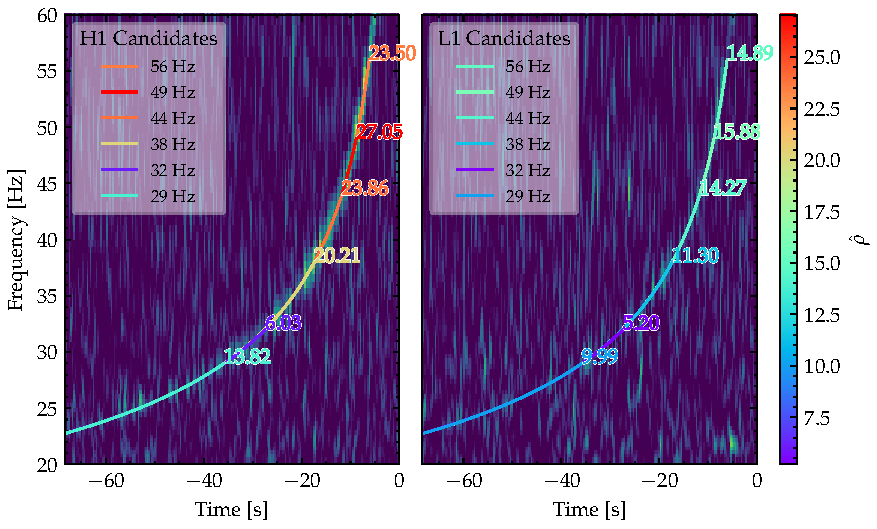
\includegraphics[width=1.0\linewidth]{images/6_earlywarning/stories/non_mono_example.pdf}
    \caption{Caption}
    \label{6:fig:non_mono_eg}
\end{figure}

It can be seen that the $32$Hz has been found by the search for this injection but with a much lower SNR than expected and not following the monotonic SNR increase that we would expect. When investigating the triggers found we can see that the search has managed to find a low-significance trigger within the coincidence time window and has managed to form a coincidence with low SNR, similar to the low significance candidates described in section~\ref{6:sec:low-significance-cands} but where one trigger is actually real. Looking into the single detector trigger files we can once again find the coicident trigger pair that should've been made if the coincidence timing window was larger and when running the search over this injection with the larger coincidence time window we find all $6$ events for this injection with the expected SNR.


% \section{\label{6:sec:potential-improvements}Potential Improvements}

% While I am not including the improvements that are suggested here into the early warning search, due to time constraints, I will delve into some of the improvements that can be made and the positives and negatives of their effect upon the search.

% \subsection{\label{6:subsec:ranking-statistic}Additions to the Ranking Statistic}

% The ranking statistic, as mentioned in previous chapters, is the way in which we can evaluate the likelihood of a particular candidate being 'real'. Therefore, if we include more and more components into the ranking statistic, we can build up a more confident picture of what determines the realness of a candidate and whether we should share this candidate with the wider research community.

% The current ranking statistic used by the early warning search is very very simple, in the single detector triggers it is a simple ranking of `newsnr' where the chi squared tests are used to determine if the correct amount of power is located in each bin of the template. For the coincident ranking statistic we used `phasetd' which is another simple check of phase and amplitude consistency between detectors in the time domain.

% We have two careful consideration with regards to the ranking statistic. Number 1, computation time and avoiding introducing any lag into the early warning search. The early warning search has a stride length of one second, if any complicate computational steps are added to the ranking statistic we might risk delaying any detected early warning candidates and defeating the purpose of the search. Number 2, eliminating potential candidates before we send them out. No ranking statistic is perfect and the resulting quantitative analysis from the ranking statistic, the false alarm rate, is cut off at a human chosen number (typically one or two per year). Therefore, if we introduce more and more complicated components to the ranking statistic we might risk eliminating early warning candidates which don't meet the PyCBC threshold of a confident event but, other non-IGWN people might take that risk and perform their observations or analyses using our non-confident predictions. Therefore we might actually want to either keep our ranking statistic fairly simple, to not lose these rare events, or lower our threshold when using a complicated ranking statistic so that we still disperse these events but with a big asterisk that we do not think they're real and might fall below someone's threshold.

% If we wanted to make some improvements to the ranking statistic we can consider including some early warning specific information which we would know at the time of the search. This is either historical information based on the previous results produced by the early warning search, something similar to the template fits used in offline and the full bandwidth live search, or maybe even an astrophysical analysis of what we expect to see based on a population model, something like the KDE statistic (I think??).

% Real time information that could be used in the search pertains to the state of the detector at that very time, inclusion of iDQ and DQ, it could also include the detected candidates that have already been found and are being kept in a rolling buffer. We do expect that for a real gravitational wave signal that can be found in early warning, to see a cascade of events uploaded with subsequent frequencies getting higher and higher. We could check if any previous frequencies were uploaded, or in posterity whether any further frequencies were uploaded. If a candidate has been found first at 38Hz, does this mean we missed a 29Hz and a 32Hz signal or were these too quiet? Can we spin up a small job to do a deep dive on whether these lower frequencies are in-fact there? There are many small changes that can be made to the early warning search to iteratively improve upon it and make it more robust and confident in detecting these rare events.

% \subsection{More Frequency Truncations per Template}
% We currently have five frequency truncations per template in our bank. This is to prevent a massive amount of templates in the bank and is a good balance for shorter templates which might transition between frequency truncations faster than the search stride time when reaching higher frequencies.

% We could produce a template bank with a number of different configurations and requirements:
% - Greater number of frequency truncations for all templates
% - Template dependent frequency truncations, longer duration templates will have more frequency truncations
% - Equal truncations per template but sigma dependent spacing
% - Time before merger spacing of templates, 1 template every 3/4/5 seconds or something. Or 8 templates per duration

% \subsection{Great parameter distribution in template bank}
% The distribution of template parameters is conservative in the early warning search. We only want to find and report on signals that have a potential electromagnetic counterpart however our template bank could be too conservative and by allowing a greater parameter distributions of templates we could discover some templates on the edge of the bank with a greater SNR or templates that previously we wouldn't have seen.

% To test a larger template bank we would need to produce an injection set containing a larger number of signals that we might consider EM bright, recent literature has highlighted previously unknown signals that could have EM counterparts~SOURCE SOURCE SOURCE.

% \subsection{Adding Spins to the Template Bank}
% Currently the template bank is limited to aligned 0 spin templates. We tested the search with an injection set of slightly spinning templates and this spin will not be seen by the early warning search. It is known that neutron stars have theoretical spins up to +-0.4 so there is a potential for us to be missing spinning neutron star signals and therefore precessing signals in our search. While precessing signals are more difficult to see due to difficulties in including the many more parameters requires this search is very light weight currently and more computing power could be added to balance out the lag increase from introducing more complicated template banks to the search.

% \subsection{Approximants with greater physics}
% Due to the small number of templates and them being only generated once for the live search we might be able to use a more expensive template model which includes physics which can capture some unique properties of low mass signals like tidal deformation or orbital eccentricity, using a better equation of state, higher order modes or high order PN terms.






%%%%%%%%%%%%%%%%%%%%%%%%%%%%%%%%%%%%%%%%%%%%%%%%%%%%%%
\section*{Appendix}
\section{Problems Faced when producing Injection Data}

One of the problems experienced while doing the data analysis of this project is an issue caused by the method of creating the data initially. The PyCBC function used was \emph{pycbc\_condition\_strain} which takes an input for the power spectrum density of the noise you with to simulate. We used an analytical PSD (NAME, REF, CITE) which produced discontinuities at the boundaries between our data segments and therefore negative effects on the matched filtering being performed by the live search. An example of one of these discontinuities and an injection missing some candidates can be seen in figure~REMOVED.
% %
% \begin{figure}
%        \centering
%     \includegraphics[width=\textwidth]{}
%     \caption{}
%     \label{fig:ew_boundary_problem}
% \end{figure}
% %
The bug can be explained by the analytical PSD not cutting off naturally when tending towards 0Hz and instead takes on values incompatible with a real PSD. This 'bug' has since been reported and a user-based solution has been found, to include a new argument to condition strain to perform a highpass on all frequencies below 10Hz. Unfortunately we did include a highpass argument on the data originall when creating the data but it was the wrong one!

Since discovering this boundary issue the same data has been re-created with the same PSD but the correct highpass argument has been given and therefore the boundary issue has been resolved and we have re-performed the initial data analysis with the new data.


\section{Existing Limitations}

\subsection{Computational Limitations}

The early warning search is heavily optimized to the point it runs on a single dedicated machine with $10$ processes and $2$ threads per process. Just as the with full bandwidth search, the template bank is parallelised over these processes using MPI so each process will be performing the matched filter for only a few hundred templates before the message passing interface receives all the results and the coicidences are found by the rank 0 process. The search can be badly affected by other processes running on the same machines so this machine is exclusively used by the PyCBC Live early warning search.

The search can suffer heavily from other non-PyCBC processes such as file storage, data frame delivery or GraceDB uploads. These can be mitigated slightly with reserved local storage on the dedicated machine or subprocess multiprocessing for the GraceDB uploads so the search isn't waiting on GraceDB to continue processing, especially at times where multiple events are being uploaded for a single signal and across multiple searches from other pipelines.

Another consideration and computational limitation is the limit in introducing new computationally complex processes to the search that might introduce lag to individual processes. Potential changes to the ranking statistic could be challenging to implement without slowing down individual processes or the coincidence rank 0 process. With a data stride of one second we need to be sure that the data processing for the current second is completed before the next second of data arrives or we will slowly build up a debt of data which the search can never get on top of.

